\documentclass[11pt,a4paper]{article}
\usepackage[margin=2.5cm]{geometry}
\usepackage[T1]{fontenc}
\usepackage[utf8]{inputenc}
\usepackage{lmodern}
\usepackage{booktabs}
\usepackage{longtable}
\usepackage{amsmath}
\usepackage{siunitx}
\usepackage{float}
\usepackage{graphicx}
\usepackage{adjustbox}
\usepackage{hyperref}
\usepackage[round,authoryear]{natbib}

\newcommand{\SuppTableInput}[1]{%
  \par
  \begingroup
  \footnotesize
  \setlength{\tabcolsep}{4pt}%
  \renewcommand{\arraystretch}{1.1}%
  \noindent\centering
  \begin{adjustbox}{max width=\linewidth}
    \input{#1}%
  \end{adjustbox}
  \par
  \endgroup
}

\title{Supporting Information: Anatomical prediction of sacroiliac motion and its load-dependent limits}
\author{Petr Heny\v{s}, Niels Hammer}
\date{}

\begin{document}
\maketitle

\section{Supplementary methods and reproducibility}
All supplementary statistics use the unloaded-subject reference $\mathbf X+\boldsymbol\phi_i$ and loaded coordinates $\mathbf X+\boldsymbol\phi_i+\mathbf u_{i\ell}$, as specified in the mathematical appendix of the main article. The three simulation variants share subject indices; resampling preserves their pairing. G denotes geometry-preserved / standardized-density (individual geometry including scale, with the spatially varying population-median density field); D denotes density-preserved / template-geometry. Full denotes individual geometry and density. The standardized density field is spatially varying, not homogeneous bone.

Component differences compare bilateral absolute magnitudes, not signed motion vectors. Their bootstrap intervals describe medians; primary tests are exact binomial sign tests. Signed-rank results are retained only as machine-readable sensitivity diagnostics. The six fully adjusted sex comparisons use HC3 covariance and a single six-test FDR family. Variance ratios are non-additive and are not causal contributions.

The conditional size-scaling model is
\begin{align}
\log Y&=\beta_0+\beta_v\log V+\beta_s\mathrm{Female}+\beta_{vs}\log V\,\mathrm{Female}\nonumber\\
&+\beta_a\mathrm{Age}_z+\beta_{AP}\mathrm{AP}_z+\beta_b\mathrm{Biischiadic}_z+\beta_p\mathrm{Subpubic}_z+\epsilon.
\end{align}
Male and female slopes are $\beta_v$ and $\beta_v+\beta_{vs}$. Conditional volume-slope tests are corrected jointly across 20 sex-specific slopes; the ten interaction tests form a separate family. Table S4 is an exact reparameterization with $\log s=(\log V-\log V_{template})/3$, so log-scale slopes equal three times the log-volume slopes. It is not an independent validation or sensitivity analysis.

The analysis comprises motion extraction, extraction sensitivity checks, statistical modeling, and generation of tables and figures. Motion is measured relative to each subject's unloaded configuration; resampling retains subject pairing across loads and model variants.


\section*{Table S1: Directional re-routing metrics}
\SuppTableInput{../tables/generated/supp_directional_rerouting.tex}

\section*{Table S2: Variance ratios and paired agreement}
\SuppTableInput{../tables/generated/supp_variance_channels.tex}
\clearpage
\subsection*{Table S2 continued: geometry-preserved/full agreement}
\SuppTableInput{../tables/generated/supp_variant_agreement.tex}

\section*{Table S3: Fully adjusted LAB sex models}
\SuppTableInput{../tables/generated/supp_sex_models.tex}

\section*{Table S4: Exact scaling reparameterization using log(scale)}
\SuppTableInput{../tables/generated/supp_allometry_scale.tex}


\clearpage
\section*{Table S5: Pooled models with subject-clustered covariance}
Coefficients with interaction terms are conditional: the volume main effect refers to male SP2leg. Outcome-SD coefficients divide by the pooled outcome SD; binary predictors retain their coding. Log-volume and the other continuous covariates are standardized. No robust-Wald statistic is interpreted as partial variance explained.
\SuppTableInput{../tables/generated/table4a_primary_models.tex}
\clearpage
\section*{Table S6: Extraction sensitivity}
Absolute differences between rigid-only and affine sacral correction in six subjects at cohort row indices 0, 55, 110, 165, 220 and 277. Each contributes five loads. These are subset maxima, not cohort-wide bounds.
\SuppTableInput{../tables/generated/supp_extraction_sensitivity.tex}
\clearpage
\section*{Age functional-form sensitivity}
A squared standardized-age term was added to each nested sex model (M0--M2) and each load-specific conditional log-volume model, retaining all other terms and HC3 covariance. This diagnostic used the same 278 subjects and did not replace the primary linear-age estimates. Adjustment for pelvic volume and the selected morphometric triad continued to attenuate translation contrasts: the maximum change in an M2 translation coefficient was 0.000334~mm, and all six M2 intervals included zero. All 20 conditional volume slopes remained negative with BH-adjusted $q\leq0.002$; the largest absolute slope change was 0.0196. Multiplicity correction used the same six-coefficient and 20-slope families as the primary analyses. These checks address age functional form, not causal mediation or equivalence.

\section*{Table S7: Sex contrasts with quadratic age adjustment}
Coefficients are female-minus-male differences in the outcome units. The M0 and M2 quadratic-age columns show the selected morphometric adjustment; the linear-age M2 column reproduces the primary model for comparison.
\SuppTableInput{../tables/generated/supp_age_sex.tex}

\clearpage
\section*{Table S8: Conditional volume slopes with quadratic age adjustment}
Slopes are dimensionless coefficients for log motion versus log total mapped bony pelvic volume. Sex-specific slopes include the sex--volume interaction and are conditional on the selected morphometric triad.
\SuppTableInput{../tables/generated/supp_age_volume.tex}

\clearpage
\section*{Table S9: Exploratory conditional log-volume slopes}
Male and female slopes use HC3 intervals. Slope $q$ values use the 20-test family; interaction $q$ values use a separate ten-test family. The models hold the selected dimensions fixed and do not describe uniformly scaled anatomies.
\SuppTableInput{../tables/generated/table4b_allometry.tex}

\clearpage
\section*{Table S10: Paired held-out prediction gains and benchmarks}
Metrics use ten repeats of ten-fold subject-held-out cross-validation, with the same folds for every load, outcome and predictor set. Size uses age and log volume; triad adds AP diameter, interspinous width and subpubic angle. Triad+sex adds female sex and its log-volume interaction. The eight-measure model uses age, log volume and all eight morphometric measures. Positive $\Delta$RMSE or percentage gain favors the augmented model. RMSE units are degrees for rotation and mm for translation. Intervals are pointwise paired subject-bootstrap intervals conditional on the fitted predictions, without refitting, feature-selection uncertainty or multiplicity adjustment.
\SuppTableInput{../tables/prediction/supp_prediction.tex}

\subsection*{Table S10 continued: Additional predictor gains and individual error}
Sex and eight-measure gains compare each benchmark with the triad. MAE and the 95th percentile of absolute error pool held-out errors across repeats for the triad model, rather than errors of repeat-averaged predictions. No benchmark gain interval is wholly positive. Nineteen of twenty intervals include zero; the remaining interval favors the triad over the sex-augmented model for SP1leg rotation.
\SuppTableInput{../tables/prediction/supp_prediction_benchmarks.tex}

\clearpage
\section*{Table S11: Density-standardization agreement and error tails}
Errors are geometry-preserved minus full-model endpoints, paired within subject and load. This simplification retains complete individual modeled geometry, including size. Mean bias is signed; the 95th percentile and maximum use absolute errors. Cohort RMSE does not bound individual error.
\SuppTableInput{../tables/prediction/supp_agreement_tails.tex}

\section*{Table S12: Direct application-site contrasts}
Contrasts are within-subject LAB2 minus LAB1 differences in bilateral absolute translation components. Pointwise percentile intervals use 3000 subject bootstrap samples. Exact two-sided sign tests are adjusted within the three-component family. These retrospective contrasts compare the sites directly, separately from their contrasts with SP2leg.
\SuppTableInput{../tables/prediction/supp_site_contrasts.tex}

\clearpage
\section*{Table S13: Effect of triad adjustment on volume slopes}
Both models use log outcome, log volume, sex, sex--volume interaction and age; the adjusted model adds the triad. Intervals use HC3 covariance. The last column applies BH correction across the 20 sex-specific slopes from the model without the triad; adjusted-model $q$ values are in Table S9. All point estimates are negative in both specifications, but precision and magnitude depend on adjustment. These conditional coefficients are distinct from held-out predictive performance.
\SuppTableInput{../tables/prediction/supp_volume_adjustment.tex}

\clearpage
\section*{Supplementary Figure S1: Raw data and adjusted curves}
\begin{center}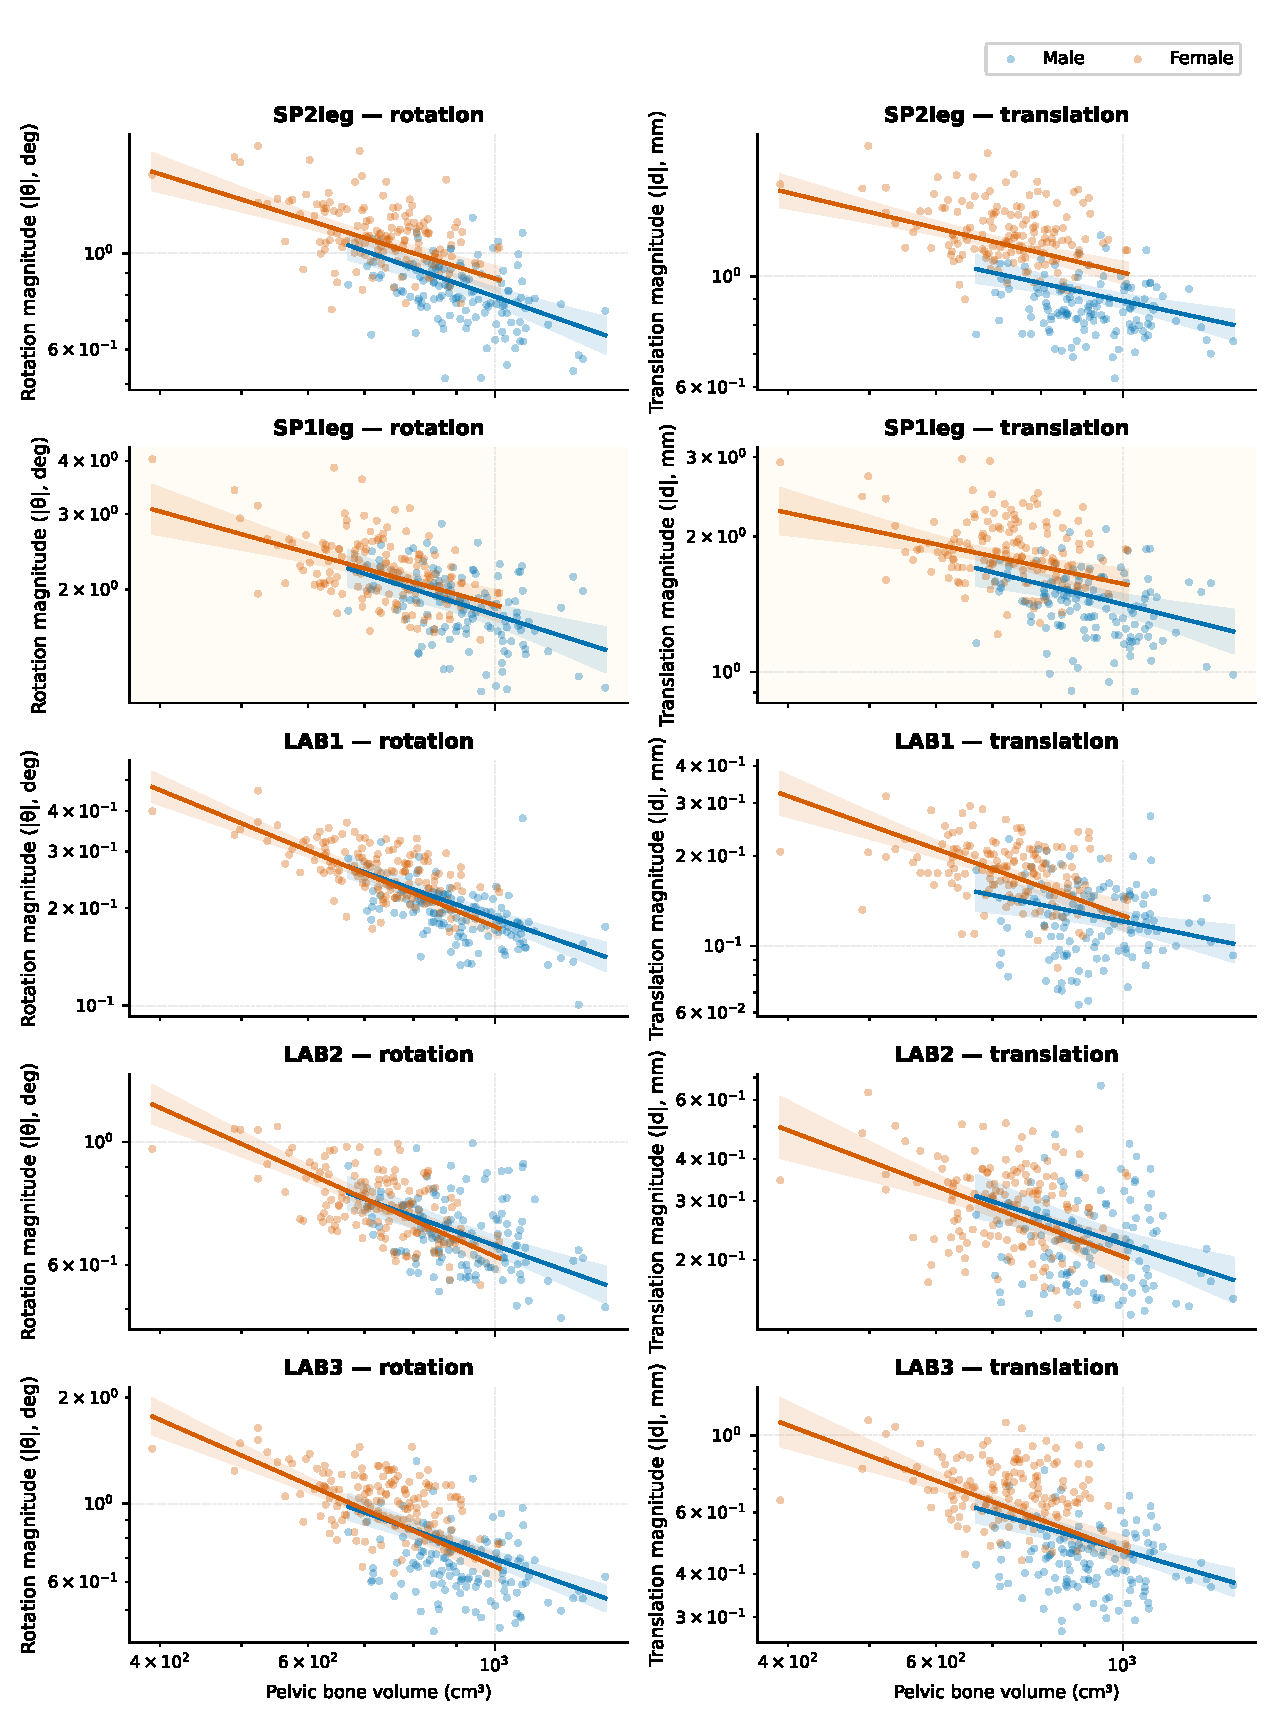
\includegraphics[width=0.94\textwidth]{../figures/SuppFig1_allometry_scatter.pdf}\end{center}
Points are raw observations. Lines and bands are conditional geometric means and pointwise HC3 95\% confidence intervals from the adjusted model, with age and the morphometric triad held at their cohort means. Thus the curves need not pass through the raw group means. Lines are restricted to each sex's observed volume range. The corresponding conditional slopes and intervals are reported in Supplementary Figure S3 and Table S9.


\clearpage
\section*{Supplementary Figure S2: Motion coordinates and geometric size}
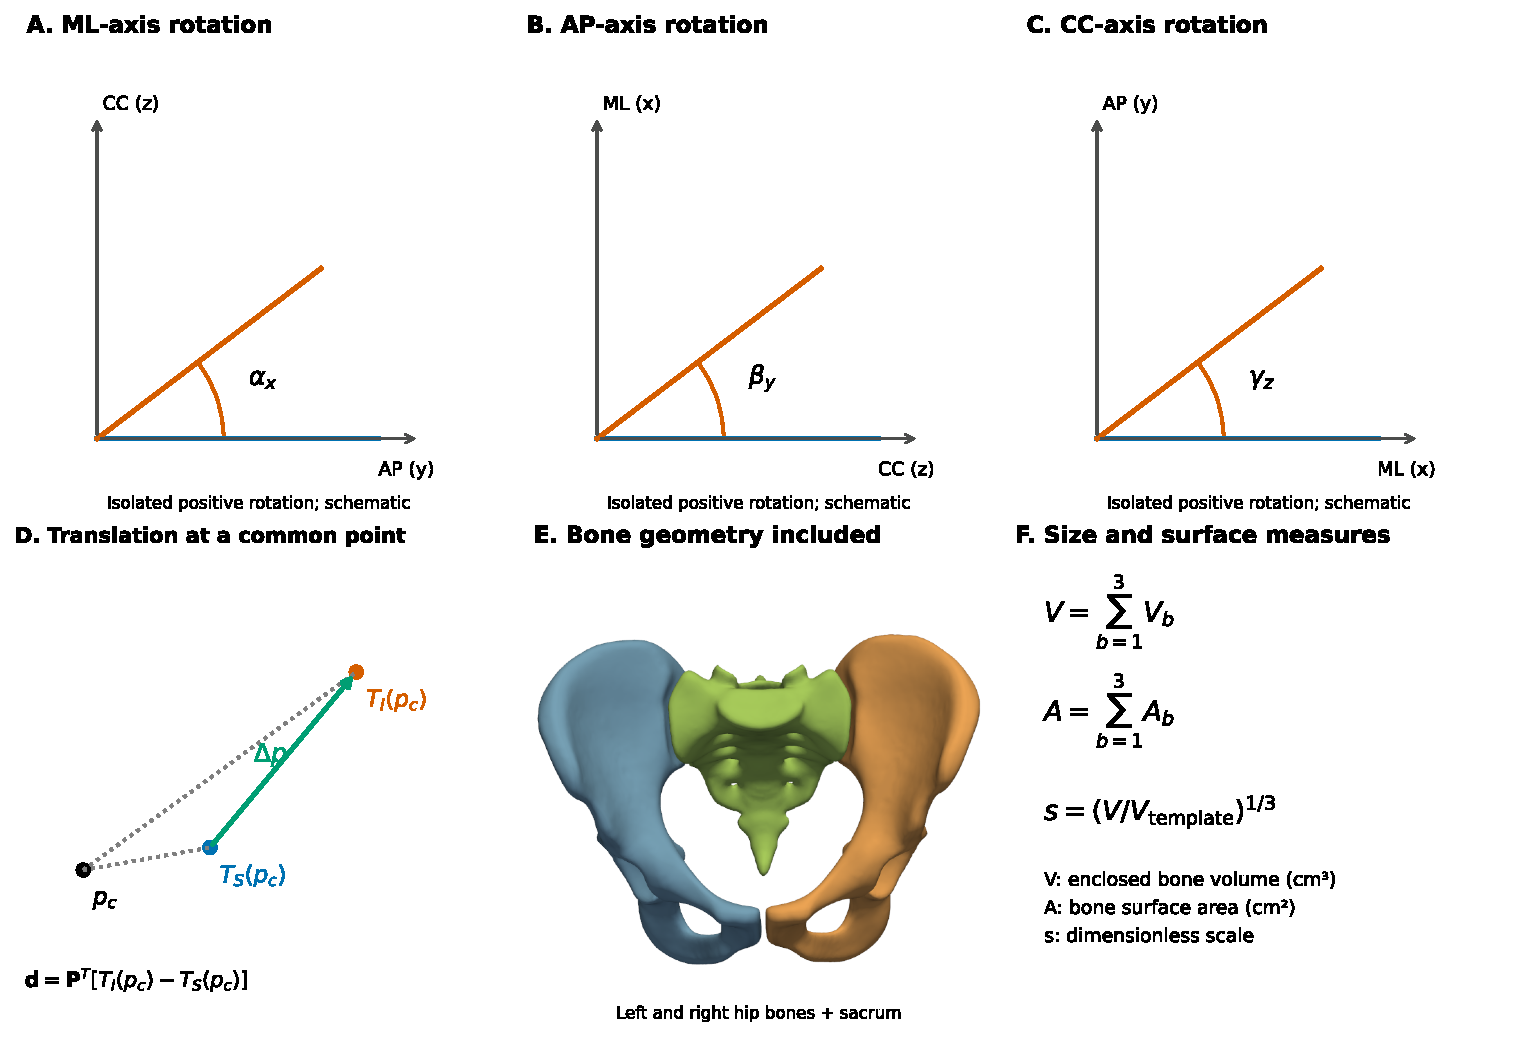
\includegraphics[width=\textwidth]{../figures/SuppFig2_measurement_conventions.pdf}
(A--C) Isolated positive rotations about the ML, AP and CC axes in a right-handed reporting frame. These schematic angles are exaggerated for clarity; the actual Cardan decomposition follows $R_z(\gamma_z)R_y(\beta_y)R_x(\alpha_x)$, rather than three independent planar angle measurements. (D) Both fitted bone maps are evaluated at the same unloaded sacral ROI centroid $p_c$; their difference is expressed in the pelvic frame. $T_I$ and $T_S$ denote the iliac and sacral rigid fits after affine correction. This is not a surface gap. (E,F) The two hip bones and sacrum define the summed enclosed bone volume and surface area; lumbar vertebrae and the space inside the pelvic canal are excluded. Scale is the cube root of the subject-to-template volume ratio. Morphometric landmark definitions are shown in main Figure 1.

\clearpage
\section*{Supplementary Figure S3: Conditional log-volume slopes}
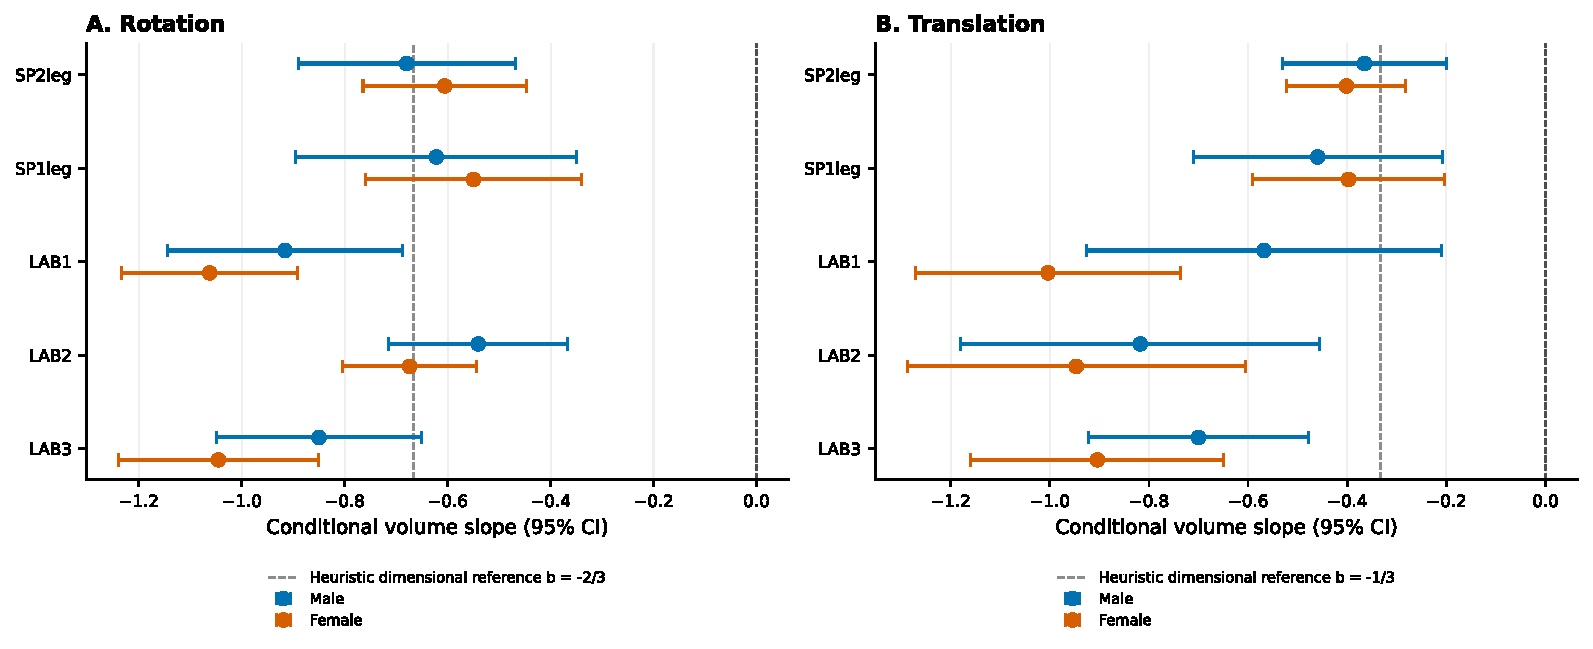
\includegraphics[width=\textwidth]{../figures/Fig6_allometry_loglog.pdf}
Male and female slopes with pointwise HC3 95\% intervals from the adjusted models in Table S9. Dashed lines at $-2/3$ (rotation) and $-1/3$ (translation) are heuristic dimensional references for geometrically similar linear-elastic structures at fixed force and modulus: $u\sim F/(EL)\propto V^{-1/3}$ and $\theta\sim u/L\propto V^{-2/3}$. They are not expected conditional regression coefficients, fitted values or tested scaling laws. The regression holds other dimensions fixed, and the model's fixed ligament stiffness and nominal tissues do not enforce geometric similarity. Numerical proximity to these references therefore provides only exploratory context. Between-load slope comparisons are descriptive. The zero line indicates no conditional association; slope tests are in Table S9.

\end{document}
